\documentclass[11pt]{article}

% ---------------------------------------------------------------------
% Packages
% ---------------------------------------------------------------------
\usepackage[margin=1in]{geometry}
\usepackage{amsmath}
\usepackage{booktabs}
\usepackage{graphicx}
\usepackage{caption}
\usepackage{subcaption}
\usepackage{xcolor}
\usepackage{enumitem}
\usepackage[numbers]{natbib}
\usepackage[colorlinks=true,linkcolor=blue!50!black,citecolor=blue!50!black,urlcolor=blue!50!black]{hyperref}

\graphicspath{{images/adult/}{images/german/}}

\title{Adaptive Alpha Control: A Trend-Aware Dynamic Weighting \\
Mechanism for Stable Adversarial Debiasing}

\author{Lewis Shearer \\ \small{Independent Research}}

\date{\today}

\hypersetup{
    pdftitle={Adaptive Alpha Control: A Trend-Aware Dynamic Weighting Mechanism for Stable Adversarial Debiasing},
    pdfauthor={Lewis Shearer},
    pdfsubject={Adversarial debiasing, fairness in machine learning},
}

\begin{document}

\maketitle

\begin{abstract}
Adversarial debiasing trains a model alongside a second ``adversary'' model
that tries to guess a sensitive attribute (such as gender) from the first
model's predictions. A single weight, usually written $\alpha$, controls how
much the main model is penalized for leaking that attribute. In the standard
approach \citep{zhang2018}, $\alpha$ is fixed by hand before training and left
unchanged. Picking it too low leaves the model biased; picking it too high
damages accuracy, and the right value is not known in advance. We introduce
\textbf{Adaptive Alpha Control}, a lightweight controller that adjusts
$\alpha$ automatically, once per training epoch, based on how accuracy and
fairness are trending. The controller smooths the recent trend in each
metric, combines the trends into a single signal, and nudges $\alpha$ up or
down accordingly, with a hard safety rule that protects accuracy if it ever
drops too far. Across 30 random seeds on the UCI Adult Income dataset, the
adaptive controller matches the best of eight hand-picked fixed $\alpha$
values on two fairness metrics, while requiring no sweep to find that value
in advance, and is noticeably more consistent from run to run. We repeat the
whole comparison on a second, much smaller dataset (German Credit) and find
the benefit shrinks but does not disappear, and we report an honest account
of a hyperparameter-tuning mistake made -- and caught -- along the way.
\end{abstract}

\tableofcontents

% =======================================================================
\section{Introduction}
% =======================================================================

Machine learning models trained on historical data can pick up and amplify
biases present in that data. A common example is income prediction: a model
trained on census data to predict whether someone earns over \$50,000 a
year can end up systematically less accurate for one gender than another,
simply because the training data reflects historical inequalities.

One well-known way to reduce this kind of bias is \textbf{adversarial
debiasing}, introduced by \citet{zhang2018}. The idea is to train two
models against each other:

\begin{itemize}[nosep]
    \item A \textbf{predictor}, which does the actual job (e.g. predicting
    income).
    \item An \textbf{adversary}, which only sees the predictor's output and
    tries to guess the sensitive attribute (e.g. gender) from it.
\end{itemize}

If the adversary can guess gender accurately just from the predictor's
output, that output must be carrying gender information it shouldn't need.
So the predictor is trained with two goals at once: get the prediction
right, \emph{and} give the adversary as little to work with as possible. A
single number, $\alpha$, controls the balance between these two goals.

The problem this paper addresses is simple to state: \emph{how do you
choose $\alpha$?} In the original method, $\alpha$ is picked once, by hand,
and held constant for the whole training run. This is a difficult choice to
get right, for two reasons. First, the best value is not known ahead of
time -- the only reliable way to find it is to train the model many times
with different values and compare the results afterwards, which is
expensive. Second, and more subtly, the \emph{right} value of $\alpha$ is
not necessarily constant even within a single training run: early in
training the adversary has little to work with, while later on, as the
predictor converges, bias can creep back in a different way. A single fixed
number is a compromise averaged over the whole run, not a value tuned to
what is actually happening at each point in training.

This paper proposes \textbf{Adaptive Alpha Control}: instead of fixing
$\alpha$, we recompute it automatically at the end of every training epoch,
based on how accuracy and two standard fairness metrics have been trending
recently. If bias is trending upward, the controller increases $\alpha$
(lean harder on the adversary). If accuracy is improving, that increase is
pulled back, so a fairness gain that would have happened anyway is not paid
for twice. If accuracy ever drops below a safe threshold, a hard override
forces $\alpha$ back down, no matter what the fairness numbers say. The
mechanism is deliberately simple -- no extra neural network, no
reinforcement learning, just a handful of smoothed running averages and one
update rule -- which keeps it easy to explain, debug, and reproduce.

\paragraph{Contributions.} In summary, this paper contributes:

\begin{enumerate}[nosep]
    \item A simple, interpretable controller that adjusts the adversarial
    weight $\alpha$ automatically during training, reacting to the
    \emph{trend} of accuracy and fairness rather than their absolute level.
    \item An explicit accuracy safety net that guarantees a worst-case
    behaviour, directly addressing the most common practical concern with
    adversarial debiasing: uncontrolled accuracy loss.
    \item A rigorous evaluation methodology: 30 random seeds per condition
    (well above the 5--10 typically used in this area), an eight-point
    sweep of fixed $\alpha$ values used as the comparison baseline (rather
    than one arbitrarily chosen value), and an analysis of both average
    outcomes \emph{and} run-to-run stability.
    \item A second, independent evaluation on a different dataset (German
    Credit), including a transparent account of a hyperparameter-tuning
    mistake that was made and subsequently caught by validating against
    more data than the original search used -- a broadly useful lesson
    beyond this specific project.
\end{enumerate}

% =======================================================================
\section{Background: Adversarial Debiasing}
% =======================================================================

We briefly summarise the method this paper builds on, following
\citet{zhang2018}, before describing our extension.

\subsection{The two models}

Both models are small, fully-connected neural networks:

\begin{itemize}[nosep]
    \item \textbf{Predictor}: takes the input features (e.g. someone's
    census record) and outputs a single number between 0 and 1, the
    predicted probability of the target outcome (e.g. income over
    \$50,000).
    \item \textbf{Adversary}: takes \emph{only} the predictor's single
    output number -- not the original features, not the true label -- and
    outputs a predicted probability of the sensitive attribute (e.g.
    gender).
\end{itemize}

Restricting the adversary to see only the predictor's output, rather than
the full input, is what makes this an adversarial \emph{debiasing} method
rather than just a second classifier: if the adversary can still guess
gender well from a single number, that number is provably leaking gender
information, since it has no other source for it.

\subsection{The training objective}

The two models are trained together. The adversary is trained normally, to
get as good as possible at guessing the sensitive attribute:
\begin{equation}
    \mathcal{L}_{\text{adv}} = \text{BCE}(z, \hat{z})
\end{equation}
where $z$ is the true sensitive attribute, $\hat z$ is the adversary's
guess, and BCE is binary cross-entropy loss (a standard way of scoring how
good a probability prediction is).

The predictor is trained to do two things at once: predict the target
correctly, \emph{and} make the adversary's job as hard as possible:
\begin{equation}
    \mathcal{L}_{\text{pred}} = \text{BCE}(y, \hat{y}) \;-\; \alpha \cdot \text{BCE}(z, \hat{z})
    \label{eq:pred-loss}
\end{equation}
where $y$ is the true target label and $\hat y$ is the predictor's output.
Subtracting the adversary's loss (scaled by $\alpha$) means the predictor is
rewarded when the adversary does \emph{badly} -- in other words, the
predictor is pushed to produce outputs the adversary cannot use to guess
gender.

$\alpha$ is the single knob that decides how much weight this fairness goal
gets relative to the accuracy goal. This is exactly the knob our method
replaces with an automatic controller.

% =======================================================================
\section{Method: Adaptive Alpha Control}
\label{sec:method}
% =======================================================================

\subsection{Overview}

Instead of a constant $\alpha$, we recompute $\alpha$ once per epoch,
using a small feedback controller. At a high level, after every epoch the
controller:

\begin{enumerate}[nosep]
    \item Measures accuracy and two fairness metrics on held-out data.
    \item Works out how much each one has moved since the previous epoch.
    \item Smooths those changes over time, so that a single noisy epoch
    does not cause an overreaction.
    \item Combines the three smoothed trends into one number, which we
    call \emph{pressure}.
    \item Moves $\alpha$ up or down based on that pressure, within fixed
    safe limits.
\end{enumerate}

This is a form of simple, interpretable feedback control: it reacts to
whether things are getting better or worse \emph{right now}, for this
particular training run, rather than following a fixed schedule decided in
advance.

\subsection{Fairness metrics}

We track two standard group-fairness metrics, computed on held-out test
data at the end of every epoch, comparing outcomes between the two values
of the sensitive attribute (referred to as group 0 and group 1):

\begin{itemize}[nosep]
    \item \textbf{Difference in Equal Opportunity (DEO)}: among people who
    actually belong to the positive class (e.g. genuinely earn over
    \$50,000), is the model equally good at correctly identifying them
    across the two groups? Formally, it is the absolute difference in true
    positive rate (TPR) between the two groups:
    \begin{equation}
        \text{DEO} = |\text{TPR}_0 - \text{TPR}_1|
    \end{equation}
    Lower is better; zero means the model catches true positives equally
    well in both groups.

    \item \textbf{Difference in Average Odds (DAO)}: a broader version of
    DEO that also checks the model does not falsely flag one group more
    than the other. It averages the true-positive-rate gap and the
    false-positive-rate (FPR) gap:
    \begin{equation}
        \text{DAO} = \frac{|\text{TPR}_0 - \text{TPR}_1| + |\text{FPR}_0 - \text{FPR}_1|}{2}
    \end{equation}
    Lower is better.
\end{itemize}

Accuracy (ACC) is simply the fraction of correct predictions on the same
held-out data.

\subsection{Tracking trends with an exponential moving average}

Raw epoch-to-epoch changes in DEO and DAO are noisy -- they bounce around
from batch sampling and the small size of the test set -- so reacting to
them directly would make $\alpha$ jitter. Instead, we track a smoothed
version of each metric's change using an exponential moving average (EMA),
a standard and cheap way to filter out short-term noise while still
following the underlying trend.

Let $\Delta x_t = x_t - x_{t-1}$ be the raw change in some metric $x$
(accuracy, DEO, or DAO) between epoch $t-1$ and epoch $t$. The smoothed
version is updated as:
\begin{equation}
    \widetilde{\Delta x}_t = \beta \cdot \Delta x_t + (1 - \beta) \cdot \widetilde{\Delta x}_{t-1}
\end{equation}
where $\beta$ is a smoothing factor between 0 and 1 (found by
hyperparameter search, see Table~\ref{tab:hparams}). A higher $\beta$ tracks
recent changes more closely; a lower $\beta$ smooths more aggressively. We
maintain one smoothed trend each for accuracy, DEO, and DAO.

\subsection{Combining trends into a pressure signal}

The three smoothed trends are combined into a single number, which we call
\emph{pressure}:
\begin{equation}
    p_t = w_{\text{DEO}} \cdot \widetilde{\Delta \text{DEO}}_t
        + w_{\text{DAO}} \cdot \widetilde{\Delta \text{DAO}}_t
        - w_{\text{ACC}} \cdot \widetilde{\Delta \text{ACC}}_t
    \label{eq:pressure}
\end{equation}

Reading this equation in plain terms:
\begin{itemize}[nosep]
    \item If DEO or DAO is \emph{increasing} (fairness getting worse),
    their terms are positive, which pushes pressure up.
    \item If accuracy is \emph{increasing} (getting better), the last term
    becomes more negative, which pulls pressure back down. This is
    deliberate: if fairness is improving on its own as accuracy improves,
    the controller should not additionally increase $\alpha$ just because
    it can -- that would be trading away accuracy for a fairness gain the
    model was already earning for free.
    \item $w_{\text{DEO}}$, $w_{\text{DAO}}$, and $w_{\text{ACC}}$ are fixed
    weights that decide how much each trend matters relative to the
    others. Like $\beta$, these were found by hyperparameter search.
\end{itemize}

\paragraph{Safety net.} If accuracy ever drops below a fixed floor
(0.84 for the Adult Income dataset), the controller ignores the equation
above entirely and forces the pressure to be strongly negative:
\begin{equation}
    p_t \leftarrow \min(p_t,\, -0.2) \quad \text{if } \text{ACC}_t < \text{ACC}_{\text{floor}}
\end{equation}
This guarantees that, regardless of what the fairness trends say, the
controller will always push $\alpha$ down (reduce pressure on the
adversary) whenever accuracy falls too low. This is a hard, unconditional
rule rather than something that emerges naturally from the weighted sum --
we discuss the implications of that design choice in
Section~\ref{sec:discussion}.

\subsection{Updating alpha}

Finally, $\alpha$ is updated once per epoch using the pressure signal,
scaled by a fixed step size $\eta$, and clipped to a safe range:
\begin{equation}
    \alpha_{t+1} = \text{clip}\big(\alpha_t + \eta \cdot p_t,\; \alpha_{\min},\; \alpha_{\max}\big)
    \label{eq:alpha-update}
\end{equation}

This is a simple proportional controller acting on the \emph{trend} of the
metrics: it moves $\alpha$ in the direction pressure indicates, by an
amount proportional to how strong that pressure is, while never letting
$\alpha$ leave a safe, pre-defined range. All of the constants in this
section -- $\eta$, $\alpha_{\min}$, $\alpha_{\max}$, $\beta$, and the three
weights in Equation~\ref{eq:pressure} -- were themselves found through a
hyperparameter search (not hand-picked), summarised in
Table~\ref{tab:hparams}.

\begin{table}[ht]
\centering
\caption{Adaptive controller hyperparameters, found via a Weights \&
Biases search on the Adult Income dataset.}
\label{tab:hparams}
\begin{tabular}{@{}ll@{}}
\toprule
\textbf{Parameter} & \textbf{Value} \\
\midrule
Initial $\alpha$ ($\alpha_{\text{init}}$)      & 0.4708 \\
Minimum $\alpha$ ($\alpha_{\min}$)             & 0.01 \\
Maximum $\alpha$ ($\alpha_{\max}$)             & 1.0048 \\
Step size ($\eta$)                              & 0.4468 \\
Accuracy floor (ACC$_{\text{floor}}$)          & 0.84 \\
EMA smoothing ($\beta$)                         & 0.3601 \\
DEO weight ($w_{\text{DEO}}$)                   & 0.6689 \\
DAO weight ($w_{\text{DAO}}$)                   & 1.9289 \\
Accuracy weight ($w_{\text{ACC}}$)             & 4.6453 \\
\bottomrule
\end{tabular}
\end{table}

% =======================================================================
\section{Experimental Setup}
% =======================================================================

\subsection{Datasets}

We evaluate on two standard tabular fairness benchmarks, both from the UCI
repository, with gender as the sensitive attribute in both cases.

\begin{itemize}[nosep]
    \item \textbf{Adult Income}: predict whether someone's annual income
    exceeds \$50,000. Roughly 45{,}000 records after removing rows with
    missing values, 99 features after one-hot encoding categorical
    columns.
    \item \textbf{German Credit}: predict whether someone is a good or bad
    credit risk. Only 1{,}000 records -- a much smaller and noisier
    dataset, used here to check whether findings from Adult Income
    generalise.
\end{itemize}

Both datasets are preprocessed identically for all conditions: rows with
missing values are dropped, categorical columns are one-hot encoded,
numeric columns are standardised, and the data is split 80/20 into
train/test sets, stratified by the target label, using the same random
split for every seed and every condition.

\subsection{Conditions compared}

We compare three ways of setting $\alpha$, all sharing the same
predictor/adversary architecture, the same preprocessing, and the same 30
random seeds (0--29):

\begin{itemize}[nosep]
    \item \textbf{Baseline}: no adversary at all -- the predictor is
    trained with no fairness objective whatsoever. This is a reference
    point showing how biased the model is with zero mitigation effort.
    \item \textbf{Fixed $\alpha$}: the adversarial game described in
    Section~\ref{sec:method}, but with $\alpha$ held constant for the whole run. We
    repeat this for eight different values of $\alpha$ (0.05, 0.1, 0.2,
    0.3, 0.4708, 0.7, 1.0, 1.5), each with all 30 seeds -- 240 runs in
    total. This traces out a full accuracy-versus-fairness trade-off
    curve (a \emph{Pareto frontier}), rather than relying on a single,
    possibly lucky or unlucky, choice of $\alpha$.
    \item \textbf{Dynamic $\alpha$ (ours)}: Adaptive Alpha Control, as
    described in Section~\ref{sec:method}.
\end{itemize}

Comparing against a single fixed $\alpha$ would not be a fair test: if that
one value happened to be a bad choice, the adaptive method would look
artificially better, and vice versa. By sweeping eight values, we can check
whether the adaptive controller matches the \emph{best achievable}
trade-off from manual tuning, not just beats one arbitrary setting.

\subsection{Why 30 seeds}

Each condition is repeated across 30 random seeds, controlling model
initialisation and batch ordering (the train/test split itself is fixed
across seeds). Thirty seeds is well above the five to ten commonly used in
this line of research, and is what makes it possible to report meaningful
averages, standard deviations, and stability comparisons rather than single
anecdotal runs.

% =======================================================================
\section{Results}
% =======================================================================

\subsection{Adult Income: accuracy and fairness}

Table~\ref{tab:adult-results} shows the mean and standard deviation of each
metric across 30 seeds, for the baseline, all eight fixed-$\alpha$
settings, and the adaptive controller.

\begin{table}[ht]
\centering
\caption{Adult Income results, mean $\pm$ standard deviation over 30 seeds
per condition. $\uparrow$ = higher is better, $\downarrow$ = lower is
better.}
\label{tab:adult-results}
\begin{tabular}{@{}lccc@{}}
\toprule
\textbf{Model} & \textbf{ACC} $\uparrow$ & \textbf{DEO} $\downarrow$ & \textbf{DAO} $\downarrow$ \\
\midrule
Baseline (no debiasing)      & 0.8453 $\pm$ 0.0014 & 0.0816 $\pm$ 0.0223 & 0.0807 $\pm$ 0.0138 \\
Fixed $\alpha=0.05$          & 0.8458 $\pm$ 0.0015 & 0.0697 $\pm$ 0.0239 & 0.0732 $\pm$ 0.0141 \\
Fixed $\alpha=0.1$           & 0.8456 $\pm$ 0.0019 & 0.0600 $\pm$ 0.0284 & 0.0682 $\pm$ 0.0168 \\
Fixed $\alpha=0.2$           & 0.8449 $\pm$ 0.0013 & 0.0513 $\pm$ 0.0248 & 0.0623 $\pm$ 0.0145 \\
Fixed $\alpha=0.3$           & 0.8448 $\pm$ 0.0015 & 0.0260 $\pm$ 0.0226 & 0.0476 $\pm$ 0.0132 \\
Fixed $\alpha=0.4708$        & 0.8444 $\pm$ 0.0016 & 0.0201 $\pm$ 0.0140 & 0.0401 $\pm$ 0.0086 \\
Fixed $\alpha=0.7$           & 0.8433 $\pm$ 0.0022 & 0.0445 $\pm$ 0.0222 & 0.0466 $\pm$ 0.0095 \\
Fixed $\alpha=1.0$           & 0.8416 $\pm$ 0.0019 & 0.0859 $\pm$ 0.0208 & 0.0605 $\pm$ 0.0090 \\
Fixed $\alpha=1.5$           & 0.8388 $\pm$ 0.0021 & 0.1349 $\pm$ 0.0266 & 0.0769 $\pm$ 0.0112 \\
\textbf{Dynamic (ours)}      & \textbf{0.8446 $\pm$ 0.0014} & \textbf{0.0236 $\pm$ 0.0183} & \textbf{0.0449 $\pm$ 0.0112} \\
\bottomrule
\end{tabular}
\end{table}

The adaptive controller clearly beats the baseline and most fixed-$\alpha$
settings on both fairness metrics, while giving up almost no accuracy. The
single closest fixed value, $\alpha=0.4708$ (which happens to be the
controller's own starting value), edges it out very slightly on DEO and
DAO alone, but at a small additional cost in accuracy -- so neither point
strictly beats the other; both sit close together on the same trade-off
curve. Figure~\ref{fig:pareto-adult} shows this trade-off directly: the
dynamic controller (marked with a star) lands right on the frontier traced
out by the fixed-$\alpha$ sweep, rather than being dominated by it.

\begin{figure}[ht]
    \centering
    
\includegraphics[width=0.8\textwidth]{pareto_frontier.png}
    \caption{Accuracy vs.\ fairness trade-off (Pareto frontier) on Adult
    Income. Each blue point is one fixed $\alpha$ value (mean over 30
    seeds); the red star is the adaptive controller. A point that is
    up-and-to-the-right of the curve would be a strict improvement over
    manual tuning; the adaptive controller instead lands on the curve
    itself, next to the best fixed values, without needing a sweep to find
    them.}
    \label{fig:pareto-adult}
\end{figure}

Figure~\ref{fig:epochs-adult} shows how the three conditions compare over
the course of training, averaged across all 30 seeds (shaded bands show the
spread across seeds).

\begin{figure}[ht]
    \centering
    \begin{subfigure}[b]{0.32\textwidth}
        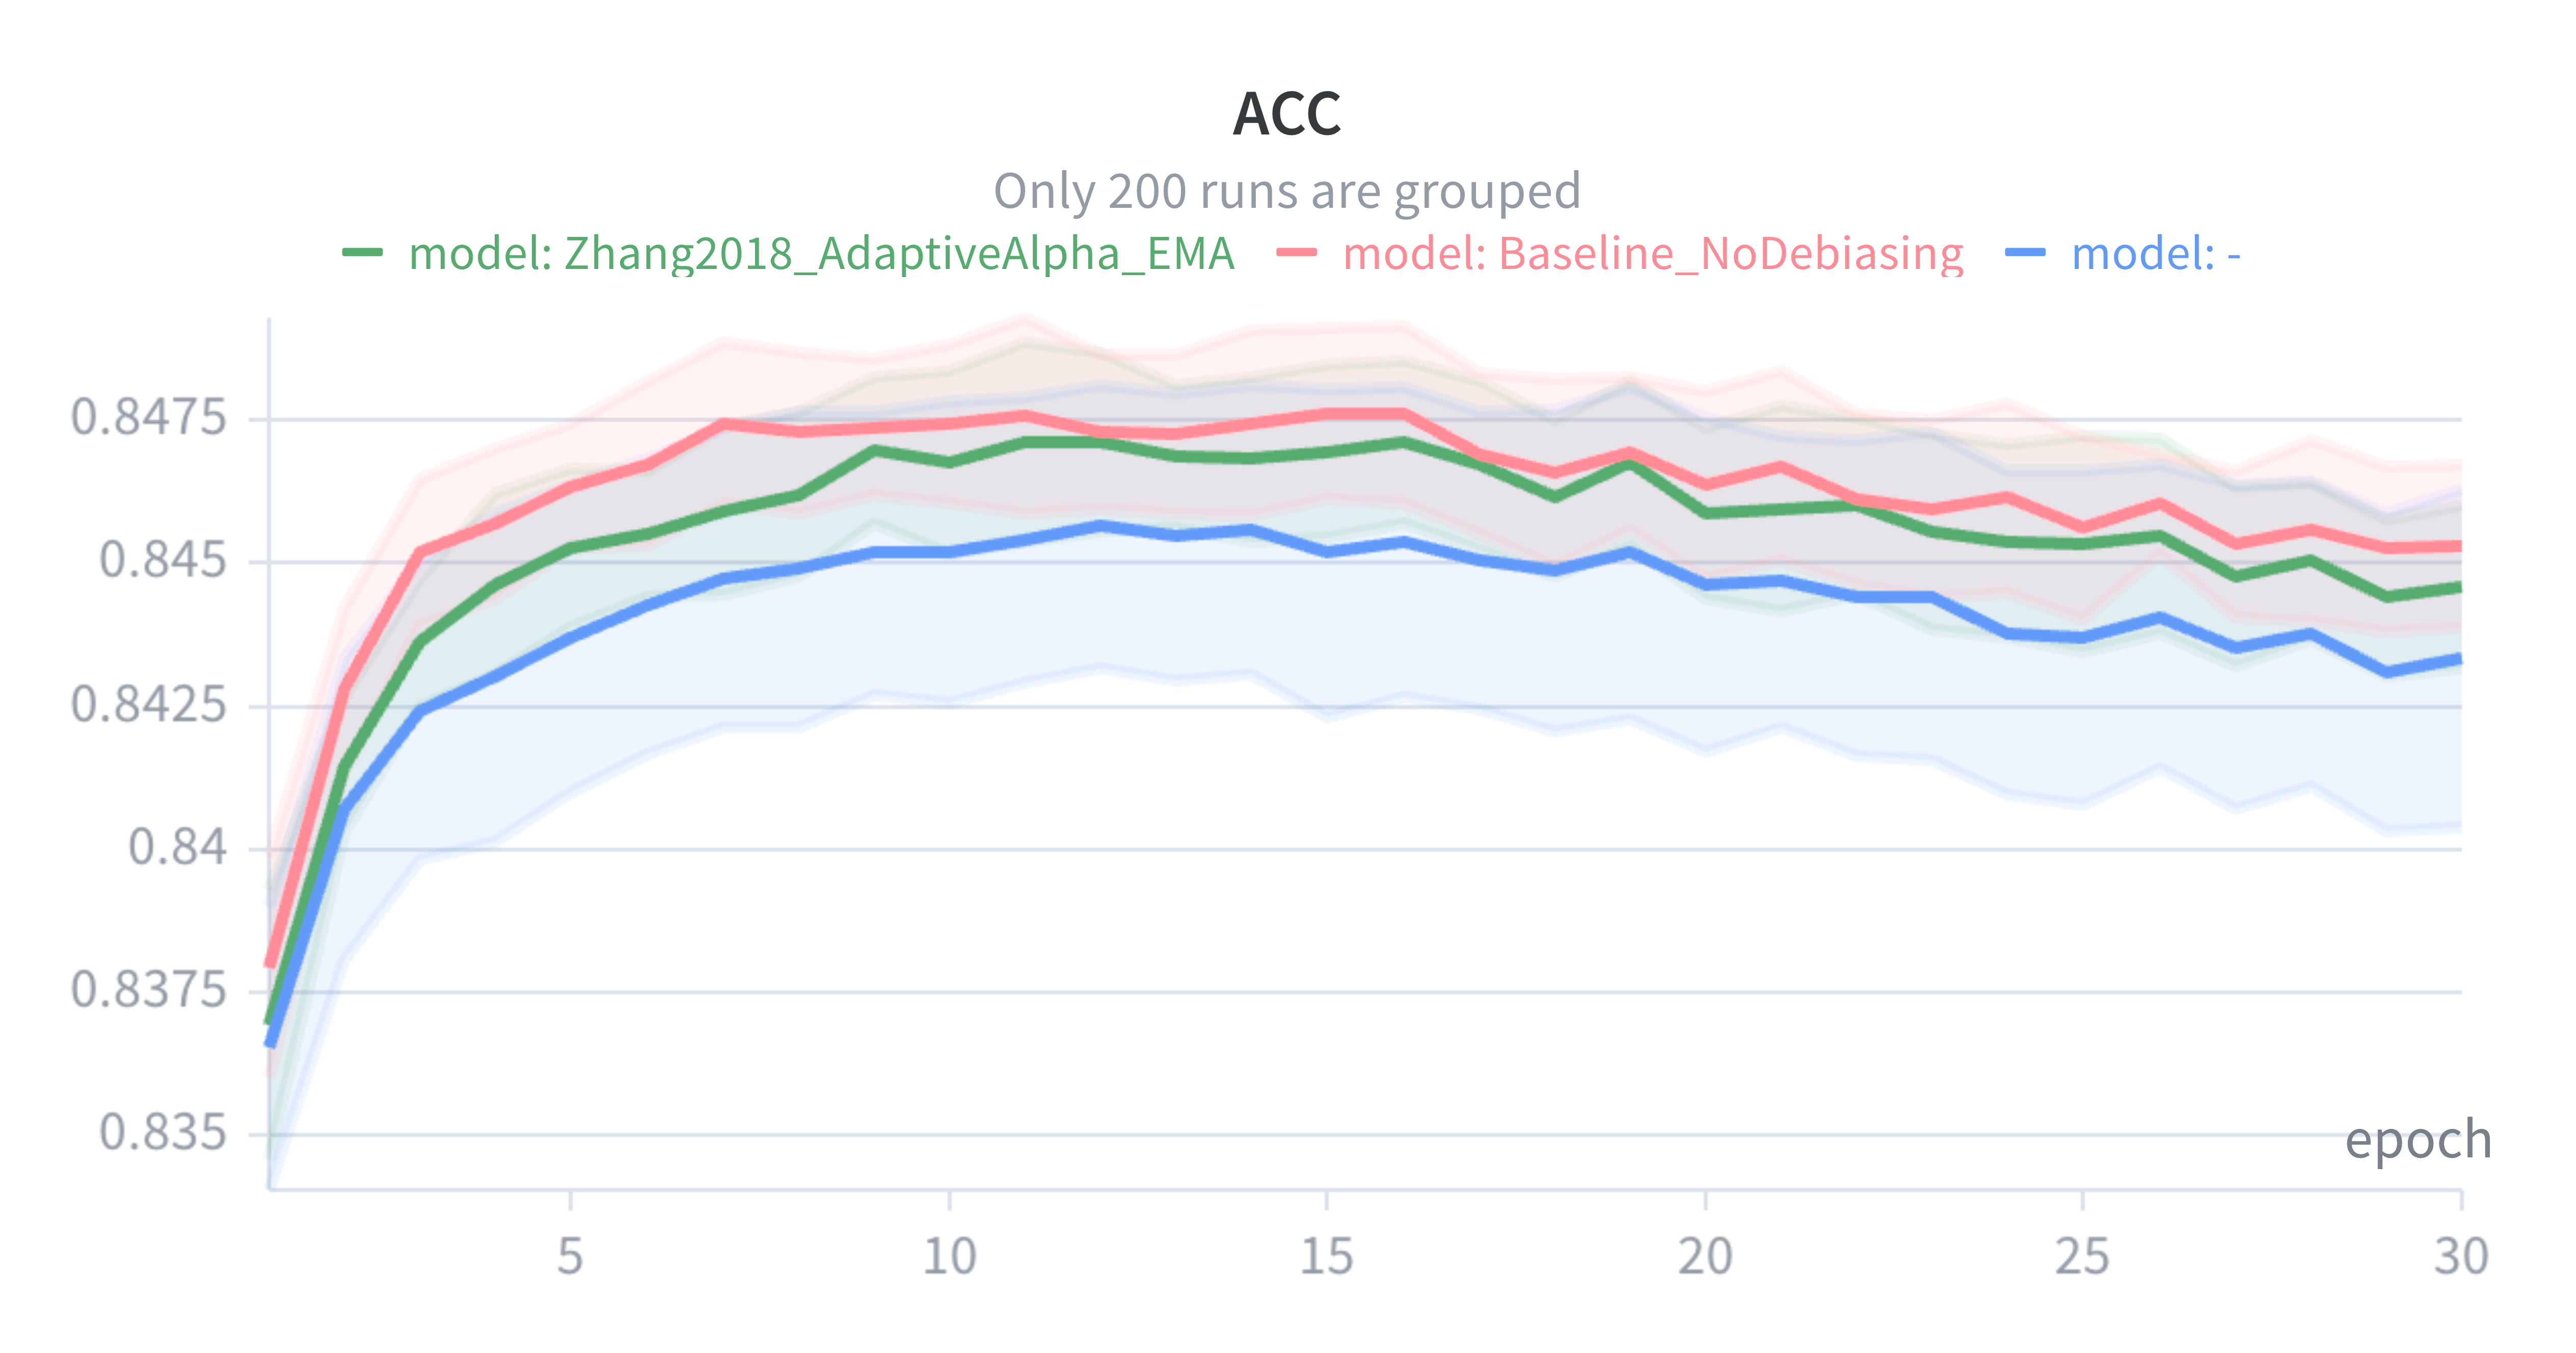
\includegraphics[width=\textwidth]{acc_over_epochs.png}
        \caption{Accuracy}
    \end{subfigure}
    \hfill
    \begin{subfigure}[b]{0.32\textwidth}
        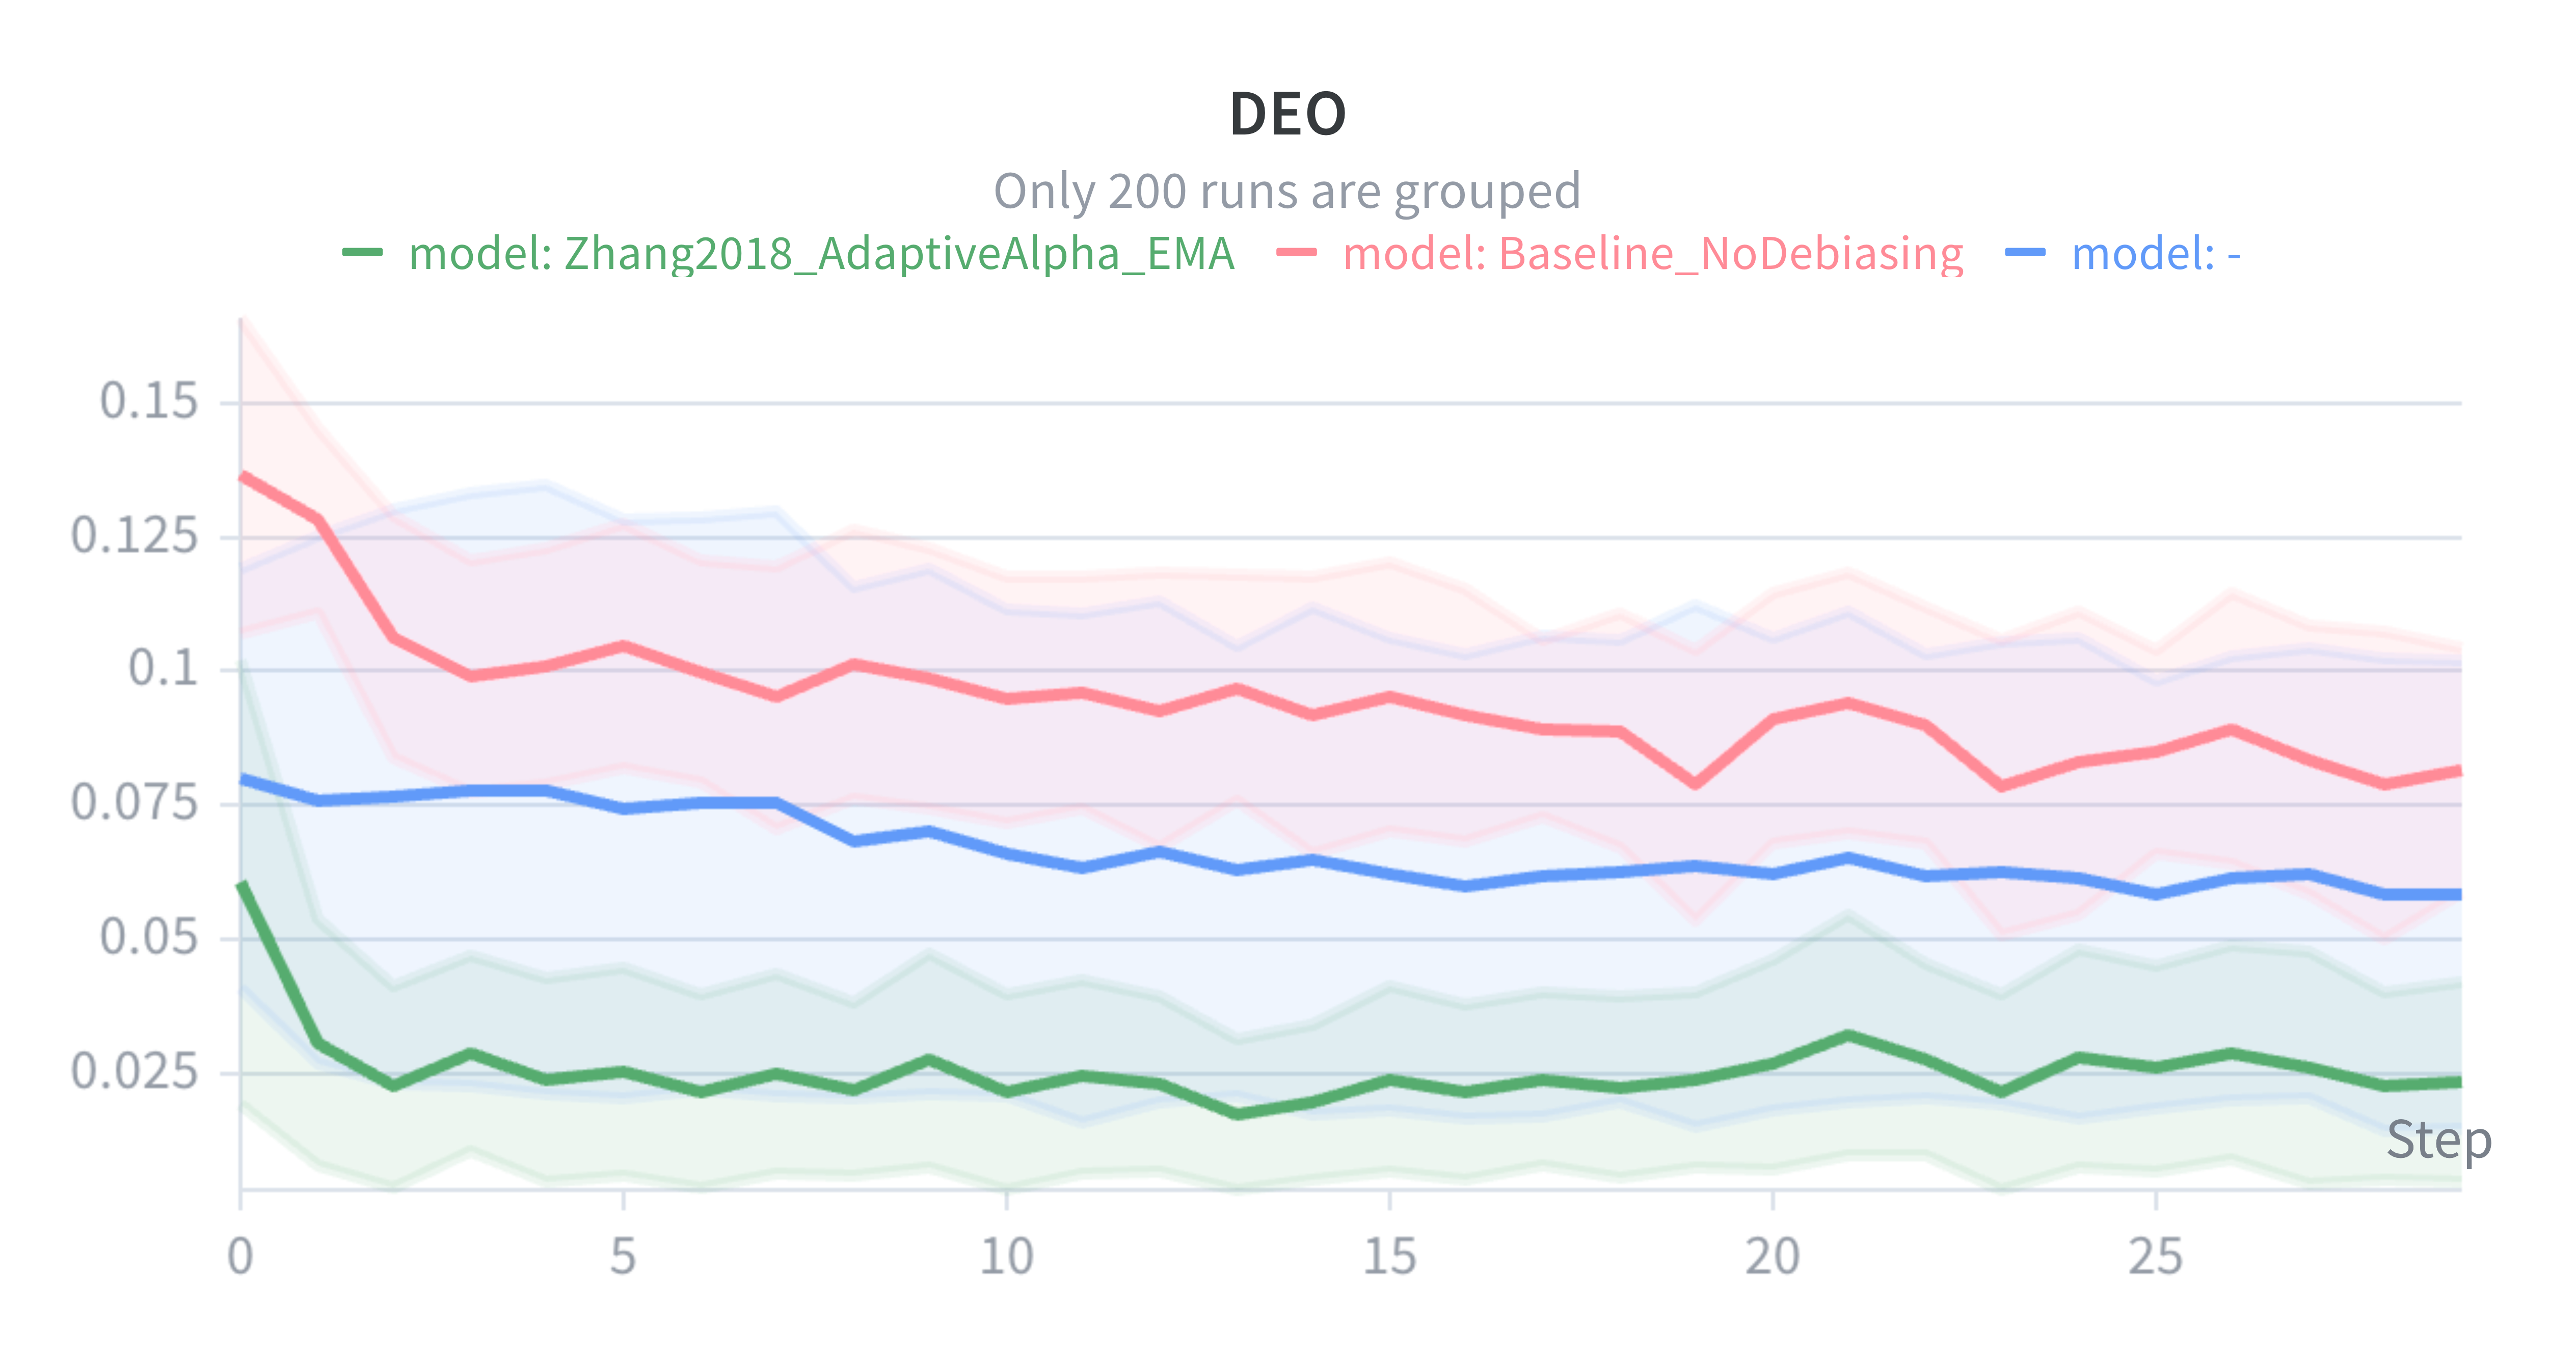
\includegraphics[width=\textwidth]{deo_over_epochs.png}
        \caption{DEO (lower is better)}
    \end{subfigure}
    \hfill
    \begin{subfigure}[b]{0.32\textwidth}
        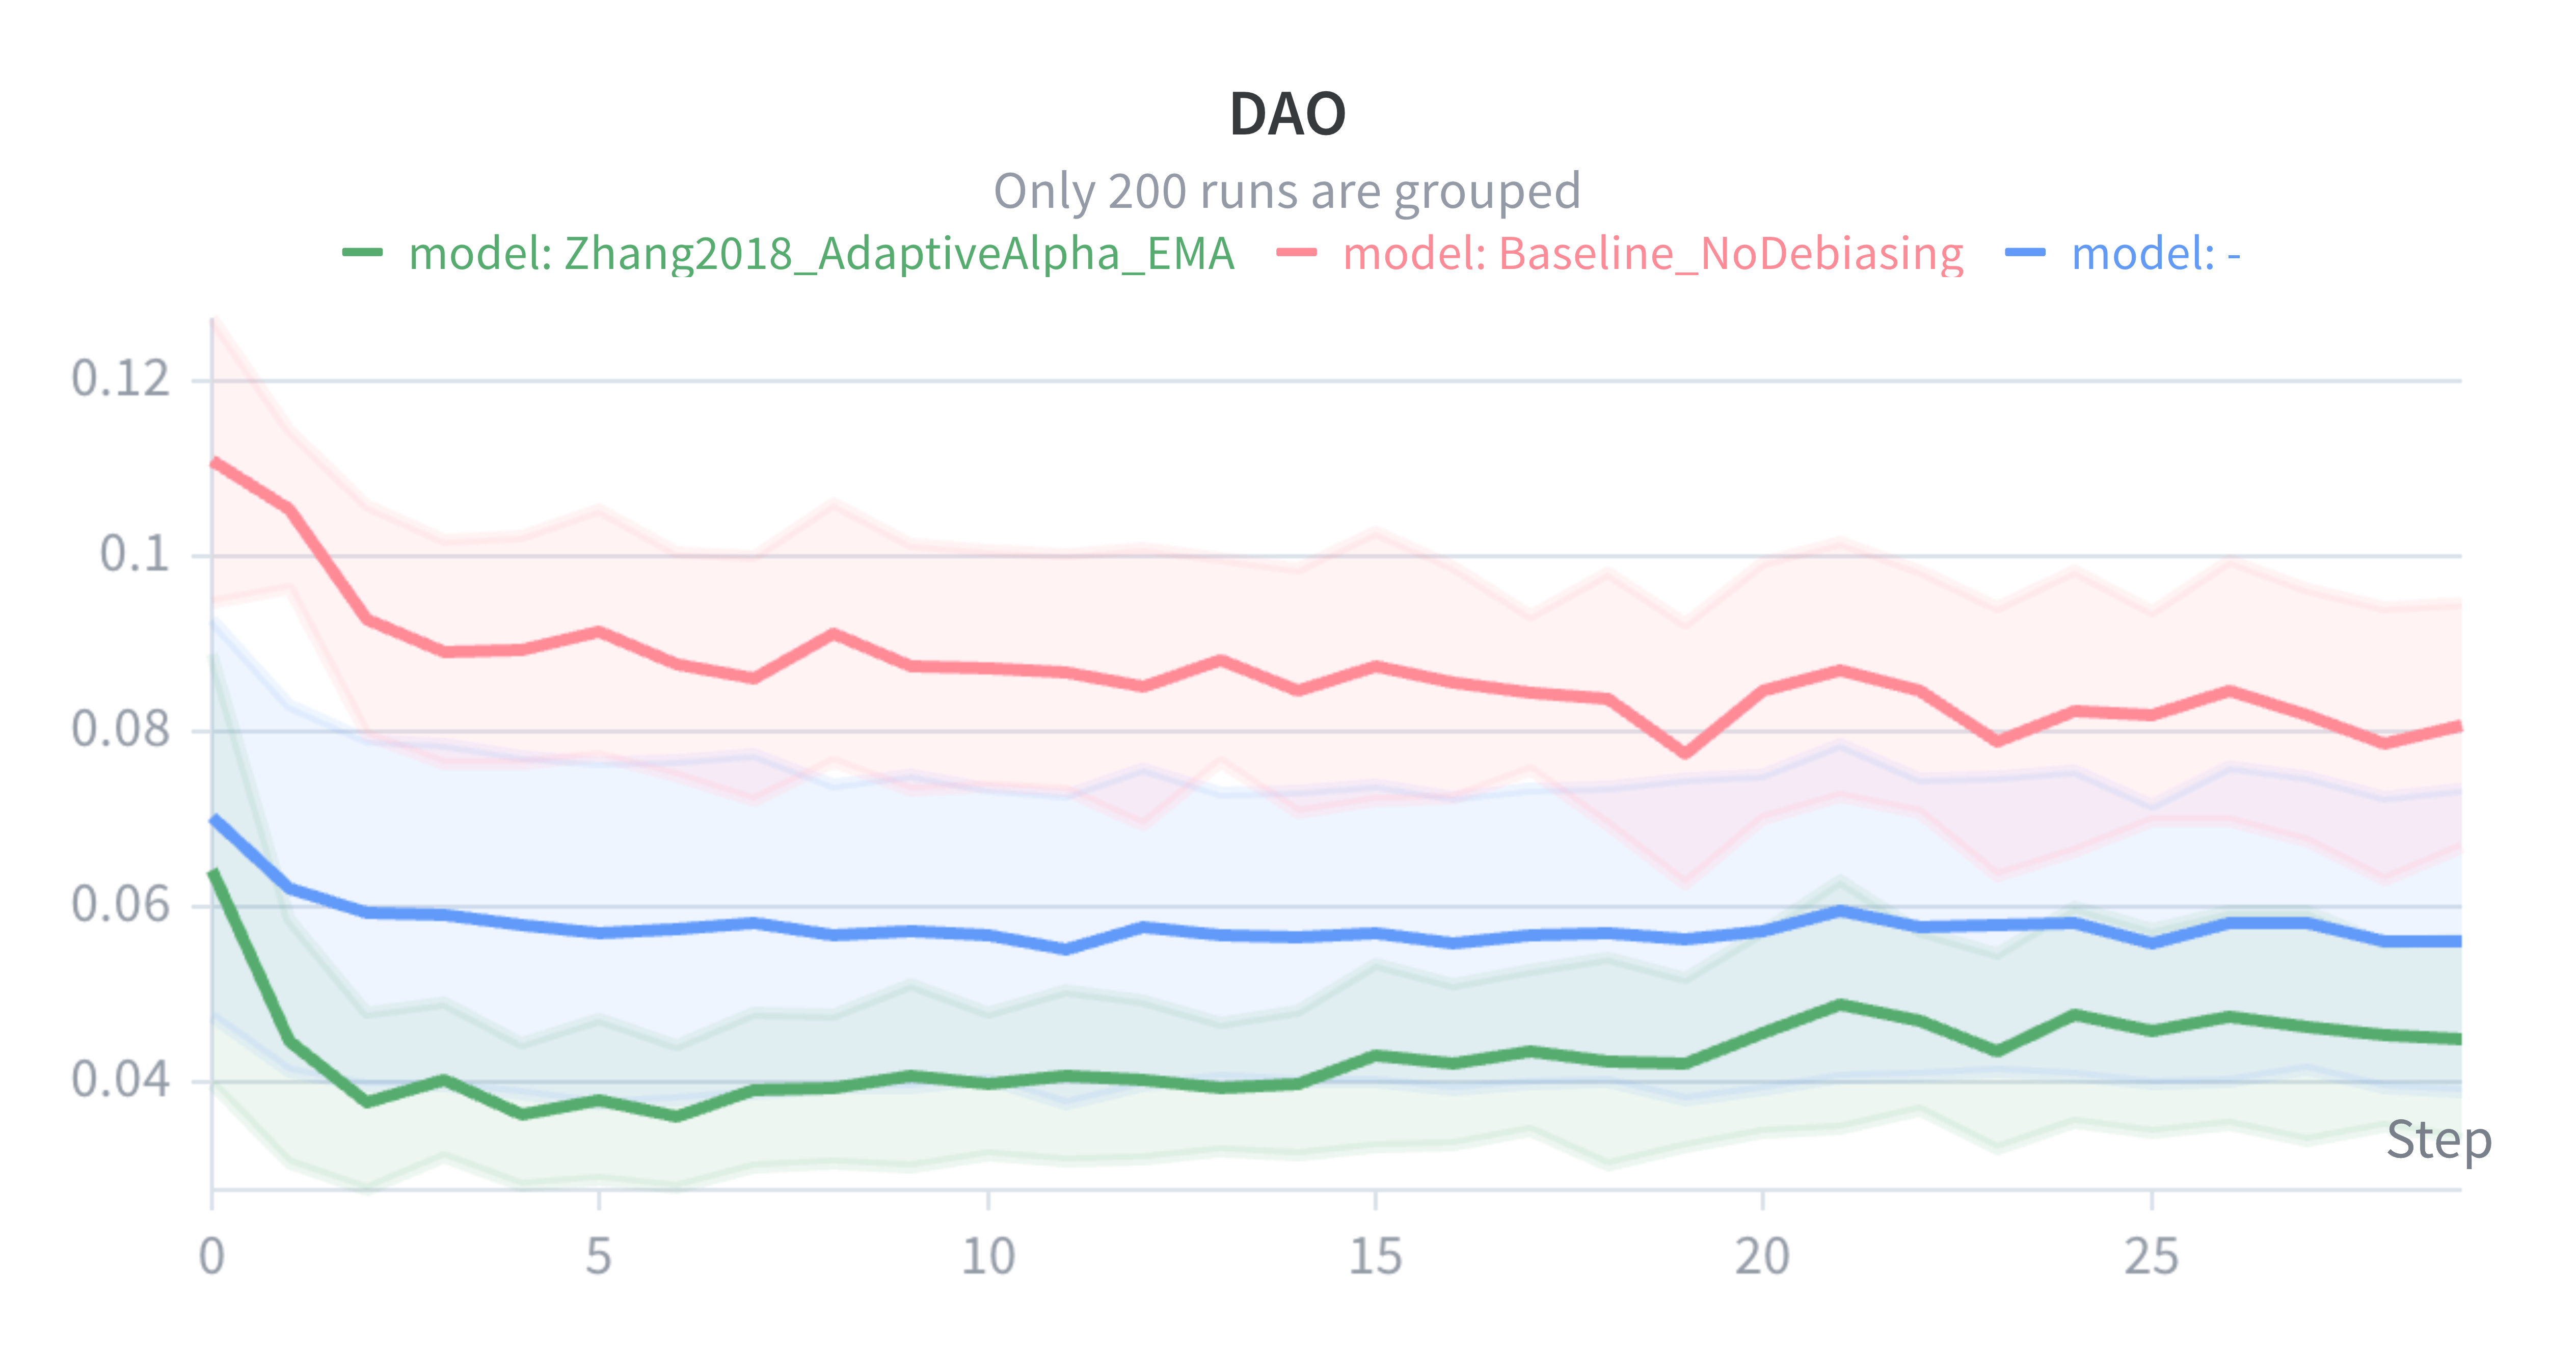
\includegraphics[width=\textwidth]{dao_over_epochs.png}
        \caption{DAO (lower is better)}
    \end{subfigure}
    \caption{Training curves over 30 epochs, averaged over 30 seeds, on
    Adult Income. Green: adaptive controller. Red: baseline. Blue:
    fixed-$\alpha$ average. The adaptive controller tracks close to the
    baseline on accuracy while dropping fastest and staying lowest on both
    fairness metrics.}
    \label{fig:epochs-adult}
\end{figure}

\subsection{Is the adaptive controller also more stable?}

A method that is good \emph{on average} but wildly inconsistent from run to
run is difficult to trust in practice. We check two different notions of
consistency, both averaged over epochs 10--30 (after the initial ramp-up
settles), using the full per-epoch history from all 30 seeds rather than
just the final-epoch summary.

\textbf{Cross-seed spread} measures how much the 30 seeds disagree with
each other at a given point in training (Table~\ref{tab:stability-spread}).

\begin{table}[ht]
\centering
\caption{Cross-seed standard deviation of each metric, epochs 10--30,
Adult Income. Lower means more consistent outcomes across random seeds.}
\label{tab:stability-spread}
\begin{tabular}{@{}lccc@{}}
\toprule
\textbf{Model} & \textbf{ACC std} & \textbf{DEO std} & \textbf{DAO std} \\
\midrule
Baseline                        & 0.0015 & 0.0238 & 0.0140 \\
Fixed $\alpha$ (average of 8)   & 0.0027 & 0.0423 & 0.0182 \\
\textbf{Dynamic (ours)}         & \textbf{0.0015} & \textbf{0.0180} & \textbf{0.0105} \\
\bottomrule
\end{tabular}
\end{table}

\textbf{Epoch-to-epoch jitter} measures how much a single run's metrics
swing from one epoch to the next (Table~\ref{tab:stability-jitter}).

\begin{table}[ht]
\centering
\caption{Average size of the epoch-to-epoch change in each metric, epochs
10--30, Adult Income. Lower means smoother, less erratic training.}
\label{tab:stability-jitter}
\begin{tabular}{@{}lccc@{}}
\toprule
\textbf{Model} & \textbf{ACC $\Delta$} & \textbf{DEO $\Delta$} & \textbf{DAO $\Delta$} \\
\midrule
Baseline                        & 0.00140 & 0.02418 & 0.01458 \\
Fixed $\alpha$ (average of 8)   & 0.00149 & 0.02290 & 0.01181 \\
\textbf{Dynamic (ours)}         & \textbf{0.00135} & \textbf{0.01872} & \textbf{0.01102} \\
\bottomrule
\end{tabular}
\end{table}

On both measures, the adaptive controller is not just competitive with
fixed $\alpha$ on average fairness -- it is genuinely more stable, both in
how much different random seeds agree with each other and in how smoothly
a single run progresses. Accuracy stability is similar across all three
conditions (the differences are small enough not to be meaningful).

\subsection{German Credit: does this generalise?}

Adult Income is a single dataset with a single sensitive attribute, so it
cannot on its own tell us whether the adaptive controller's advantage is a
general pattern or specific to this dataset. We repeat the entire
comparison on the much smaller German Credit dataset (1{,}000 rows,
predicting credit risk, gender as the sensitive attribute).

\paragraph{The controller needed re-tuning.} The hyperparameters in
Table~\ref{tab:hparams} were tuned specifically for Adult Income, and did
not transfer directly. German Credit's best achievable accuracy is only
around 73--75\%, well below the 0.84 accuracy floor tuned for Adult Income
-- so that floor was never reached, the safety override fired on
\emph{every single epoch}, and $\alpha$ collapsed to its minimum almost
immediately. A first attempt at fixing this with a small hyperparameter
search (3 seeds per trial) found a floor of 0.7366 that looked reasonable,
but validating the winning setting against the full 30 seeds revealed the
override was still firing on 84.6\% of all epochs -- the search had picked
a floor that happened to look fine against a small, noisy sample, not one
that actually solved the problem. Widening the search (8 seeds per trial)
and correcting the search range found a floor of 0.6802, which reduced the
override rate to 16.2\% of epochs, concentrated in the early part of
training rather than throughout. We report this in full because it is a
useful, generalisable lesson independent of this specific project: a
hyperparameter search's winning configuration is a claim, not a fact, and
should be validated against more data than the search itself used before
it is trusted.

\begin{table}[ht]
\centering
\caption{German Credit results (validated controller configuration), mean
$\pm$ standard deviation over 30 seeds (240 runs for the fixed-$\alpha$
sweep).}
\label{tab:german-results}
\begin{tabular}{@{}lccc@{}}
\toprule
\textbf{Model} & \textbf{ACC} $\uparrow$ & \textbf{DEO} $\downarrow$ & \textbf{DAO} $\downarrow$ \\
\midrule
Baseline (no debiasing)   & 0.7233 $\pm$ 0.0149 & 0.0893 $\pm$ 0.0370 & 0.0738 $\pm$ 0.0353 \\
Fixed $\alpha=0.05$       & 0.7253 $\pm$ 0.0180 & 0.0967 $\pm$ 0.0447 & 0.0804 $\pm$ 0.0290 \\
Fixed $\alpha=0.1$        & 0.7268 $\pm$ 0.0130 & 0.0870 $\pm$ 0.0436 & 0.0664 $\pm$ 0.0285 \\
Fixed $\alpha=0.2$        & 0.7260 $\pm$ 0.0163 & 0.0980 $\pm$ 0.0477 & 0.0815 $\pm$ 0.0412 \\
Fixed $\alpha=0.3$        & 0.7220 $\pm$ 0.0180 & 0.0908 $\pm$ 0.0515 & 0.0775 $\pm$ 0.0408 \\
Fixed $\alpha=0.4708$     & 0.7202 $\pm$ 0.0163 & 0.0920 $\pm$ 0.0455 & 0.0902 $\pm$ 0.0372 \\
Fixed $\alpha=0.7$        & 0.7253 $\pm$ 0.0176 & 0.0912 $\pm$ 0.0498 & 0.0743 $\pm$ 0.0358 \\
Fixed $\alpha=1.0$        & 0.7285 $\pm$ 0.0175 & 0.0742 $\pm$ 0.0374 & 0.0667 $\pm$ 0.0277 \\
Fixed $\alpha=1.5$        & 0.7232 $\pm$ 0.0160 & 0.0703 $\pm$ 0.0432 & 0.0635 $\pm$ 0.0345 \\
\textbf{Dynamic (ours)}   & \textbf{0.7265 $\pm$ 0.0153} & \textbf{0.0835 $\pm$ 0.0483} & \textbf{0.0755 $\pm$ 0.0393} \\
\bottomrule
\end{tabular}
\end{table}

With the corrected configuration, the adaptive controller beats the
baseline on both accuracy (0.7265 vs.\ 0.7233) and DEO (0.0835 vs.\
0.0893), and is essentially tied on DAO (0.0755 vs.\ 0.0738). It is
dominated by only one fixed value on DEO ($\alpha=1.0$) and two on DAO
($\alpha=0.1$ and $\alpha=1.0$) -- a much closer result than the broken
configuration produced, though not quite as clean a win as on Adult Income.
Unlike Adult Income, we did not observe a stability advantage on German
Credit -- cross-seed spread and epoch-to-epoch jitter were statistically
similar across all three conditions, most likely because German Credit's
much smaller test set (roughly 200 rows) makes every metric noisier to
begin with. Figure~\ref{fig:pareto-german} shows the corresponding
trade-off plot.

\begin{figure}[ht]
    \centering
    
\includegraphics[width=0.8\textwidth]{images/german/pareto_frontier.png}
    \caption{Accuracy vs.\ fairness trade-off on German Credit, using the
    corrected controller configuration. The dynamic controller sits closer
    to the fixed-$\alpha$ frontier than the broken configuration did, but
    the picture is noisier overall than on Adult Income, reflecting the
    much smaller dataset.}
    \label{fig:pareto-german}
\end{figure}

% =======================================================================
\section{Discussion}
\label{sec:discussion}
% =======================================================================

\paragraph{What the results actually show.} The adaptive controller does
not strictly dominate every fixed value of $\alpha$ -- on Adult Income, the
single fixed value equal to the controller's own starting point
($\alpha=0.4708$) is very slightly better on DEO and DAO alone, at a small
accuracy cost. The honest claim is not ``adaptive beats everything,'' but
``adaptive reaches the same operating point on the fairness--accuracy
trade-off curve that a practitioner would otherwise have to run an
eight-value sweep to find, without needing to run that sweep.'' That is a
practical, real saving in effort and compute, even though it is a more
modest claim than outright dominance.

\paragraph{The accuracy floor is a design choice, not a discovery.} Because
the controller has a hard rule that forces $\alpha$ down whenever accuracy
drops below a threshold, the fact that accuracy stays close to the baseline
across all our results is, to some extent, an engineered guarantee rather
than something that emerged naturally from the trend-aware mechanism alone.
We think this is a reasonable and honest design choice -- it is exactly
the kind of safety property a practitioner would want -- but it should be
stated plainly rather than presented as a surprising finding.

\paragraph{Dataset size matters.} The clearest result -- a genuine
stability advantage, not just a comparable average -- appeared on Adult
Income (45{,}000 rows) but not on German Credit (1{,}000 rows). This
suggests the benefit of trend-aware smoothing may depend on having enough
data for the per-epoch metrics to be measured reliably in the first place;
with a noisier signal to begin with, there may simply be less genuine
signal for the controller to react to. We see this as an open question
rather than a settled conclusion (Section~\ref{sec:limitations}).

% =======================================================================
\section{Limitations and Ethical Considerations}
\label{sec:limitations}
% =======================================================================

Adaptive Alpha Control improves the specific fairness metrics it is
measured against; it does not guarantee fairness in any broader sense.
Several limitations are worth stating plainly:

\begin{itemize}[nosep]
    \item \textbf{Binary sensitive attribute.} Gender is treated as binary
    in both datasets used here, because that is how the underlying UCI
    datasets record it. This is a limitation of the data, not an
    endorsement of that framing, and the method has not been tested with
    non-binary or multi-valued sensitive attributes.
    \item \textbf{Narrow fairness definitions.} DEO and DAO are two
    specific, widely-used definitions of group fairness. They do not
    capture every notion of what ``fair'' means (for example, individual
    fairness or calibration across groups), and improving them does not
    imply fairness has been achieved in a broader sense.
    \item \textbf{Single sensitive attribute at a time.} Both datasets test
    one sensitive attribute in isolation. Real-world settings often
    involve multiple, overlapping protected attributes, which this
    method has not been evaluated against.
    \item \textbf{Two datasets is not generality.} Testing on Adult Income
    and German Credit is enough to show the benefit is not an artifact of
    one specific dataset, but not enough to claim the method works well
    across domains or dataset sizes in general -- particularly given that
    the stability advantage did not replicate on the smaller dataset.
    \item \textbf{The controller's own hyperparameters were tuned via
    search.} The values in Table~\ref{tab:hparams} come from the same kind
    of hyperparameter search used to justify the fixed-$\alpha$ comparison
    values, which is a fair comparison of effort, but it does mean the
    controller has not been shown to work well across a wide range of its
    own hyperparameters -- only at the specific setting found by search.
    A sensitivity analysis across that range would be a natural next step
    to strengthen this claim.
    \item \textbf{Historical data carries historical bias.} Both datasets
    are drawn from historical records, which reflect the social and
    economic conditions of when they were collected. Reducing DEO/DAO on
    such data reduces one measurable symptom of that history; it does not
    correct the underlying conditions that produced it.
\end{itemize}

This work should be read as a tool for reducing one measurable form of
bias in a specific, well-defined setting, not as a general or complete
solution to fairness in machine learning.

% =======================================================================
\section{Conclusion}
% =======================================================================

We presented Adaptive Alpha Control, a simple feedback controller that
replaces the fixed, hand-tuned weighting parameter in adversarial
debiasing with an automatic, trend-aware update rule. Across 30 seeds on
the Adult Income dataset, the controller reaches the same
fairness--accuracy trade-off that would otherwise require sweeping eight
different fixed values by hand, and does so more consistently from run to
run than either the baseline or the fixed-$\alpha$ average. On a second,
much smaller dataset, German Credit, the same overall pattern holds in a
weaker form, alongside a transparent account of a hyperparameter-tuning
mistake that a naive port of settings from one dataset to another produced,
and how validating against more data caught and fixed it. We believe both
the method itself and the honest reporting of what does and does not
transfer between datasets are useful contributions for anyone building on
adversarial debiasing in practice.

\section*{Reproducibility}

All training code, preprocessing, model architectures, and Weights \&
Biases logs used in this paper are shared publicly, with all three
conditions (baseline, fixed-$\alpha$ sweep, dynamic controller) using
identical preprocessing, architecture, and random seeds, so that
differences in results can be attributed to the $\alpha$ mechanism alone
and not to confounding factors such as unequal compute budgets.

% =======================================================================
% Bibliography
% =======================================================================
\begin{thebibliography}{9}

\bibitem[Zhang et~al.(2018)]{zhang2018}
Zhang, B.~H., Lemoine, B., \& Mitchell, M. (2018).
\textit{Mitigating Unwanted Biases with Adversarial Learning}.
Proceedings of the AAAI/ACM Conference on AI, Ethics, and Society.

\end{thebibliography}

\end{document}